\chapter{引言}%
\label{chap:introduction}

自从爱因斯坦发现广义相对论以来,人类对宇宙的探索获得了前所未有的理论武器。爱因斯坦在提出广义相对论之后,很快以爱因斯坦方程为基础建立了宇宙学静态模型。1924年弗里德曼发表的文章\citep{friedmann1924moglichkeit}中正式提出了膨胀宇宙模型,基于在爱因斯坦场方程中找到的一个动态解,描述均匀且各项同性宇宙的Friedmann–Lemaître–Robertson–Walker
(FLRW)度规。
1929年哈勃依据对河外星系退行速度的观测数据提出了哈勃定律——遥远星系的退行速度与它们和地球的距离成正比\citep{hubble1929relation}。基于观测数据的哈勃定律提出后,爱因斯坦意识到自己为了获得静态宇宙模型而加入的宇宙学常数$\Lambda$是他“一生中最大的错误”。
在弗里德曼的膨胀宇宙模型以及哈勃定律的基础上,曾出现过各种非主流宇宙模型,例如米尔恩宇宙\citep{milne1936relativity}、弗里德曼提出并由爱因斯坦推广的振荡宇宙、弗里茨$\cdot$兹威基的衰减光子假说\citep{zwicky1929redshift}。
到了40年代,主要有两个基于膨胀宇宙的对立理论。一是由勒梅特提出,乔治$\cdot$伽莫夫支持并完善的热大爆炸理论,另外一个弗雷德$\cdot$霍伊尔等人提出的稳态理论\citep{hoyle1948new}。
伽莫夫在1948年发表的原初核合成理论\citep{alpher1948origin}定量描述了宇宙早期形成的氢元素丰度。另外,伽莫夫的同事拉尔夫$\cdot$阿尔菲和罗伯特$\cdot$赫尔曼从理论上预言了宇宙微波背景辐射(CMB)的存在\citep{alpher1948evolution}。
原初核合成理论的成功以及1964年宇宙微波背景的发现和确认\citep{penzias1965measurement}使得热大爆炸理论胜出。
后来越来越多的实验观测支持存在暗物质\citep{zwicky1933rotverschiebung,zwicky1937masses,clowe2006direct,rubin1980rotational}和暗能量\citep{peebles2003cosmological}。
在热大爆炸理论的基础上加入暗物质和暗能量就得到了现在的标准宇宙学模型,即$\Lambda$CDM模型。$\Lambda$CDM模型包含六个基本参数,能很好的解释宇宙膨胀、宇宙微波背景辐射、宇宙大尺度结构以及物质起源。
但是仍然存在一些根本性问题无法得到解释,如视界疑难\citep{kolb1988early}、平坦性疑难\citep{dicke1979big}等。

为了解决这些问题,Guth\citep{guth1981inflationary}在1981年首次提出了暴胀的概念,认为在宇宙极早期应存在一个短暂的加速膨胀过程,膨胀结束之后直到如今则有标准宇宙学模型进行描述。
在暴胀过程开始之前,目前的整个可观测宇宙都处在一个均匀且各项同性的区域之内。随后在暴胀的作用下,这片区域开始加速膨胀。膨胀的速度是如此之快以至于在暴胀结束之后,这块区域的尺度远远超过了当时的可观测宇宙的尺度。

标准宇宙学模型加上暴胀理论对宇宙演化的描述基本如图$(\ref{fig:history-of-universe})$所描述的样子。

\begin{figure*}[!htbp]
  \centering
  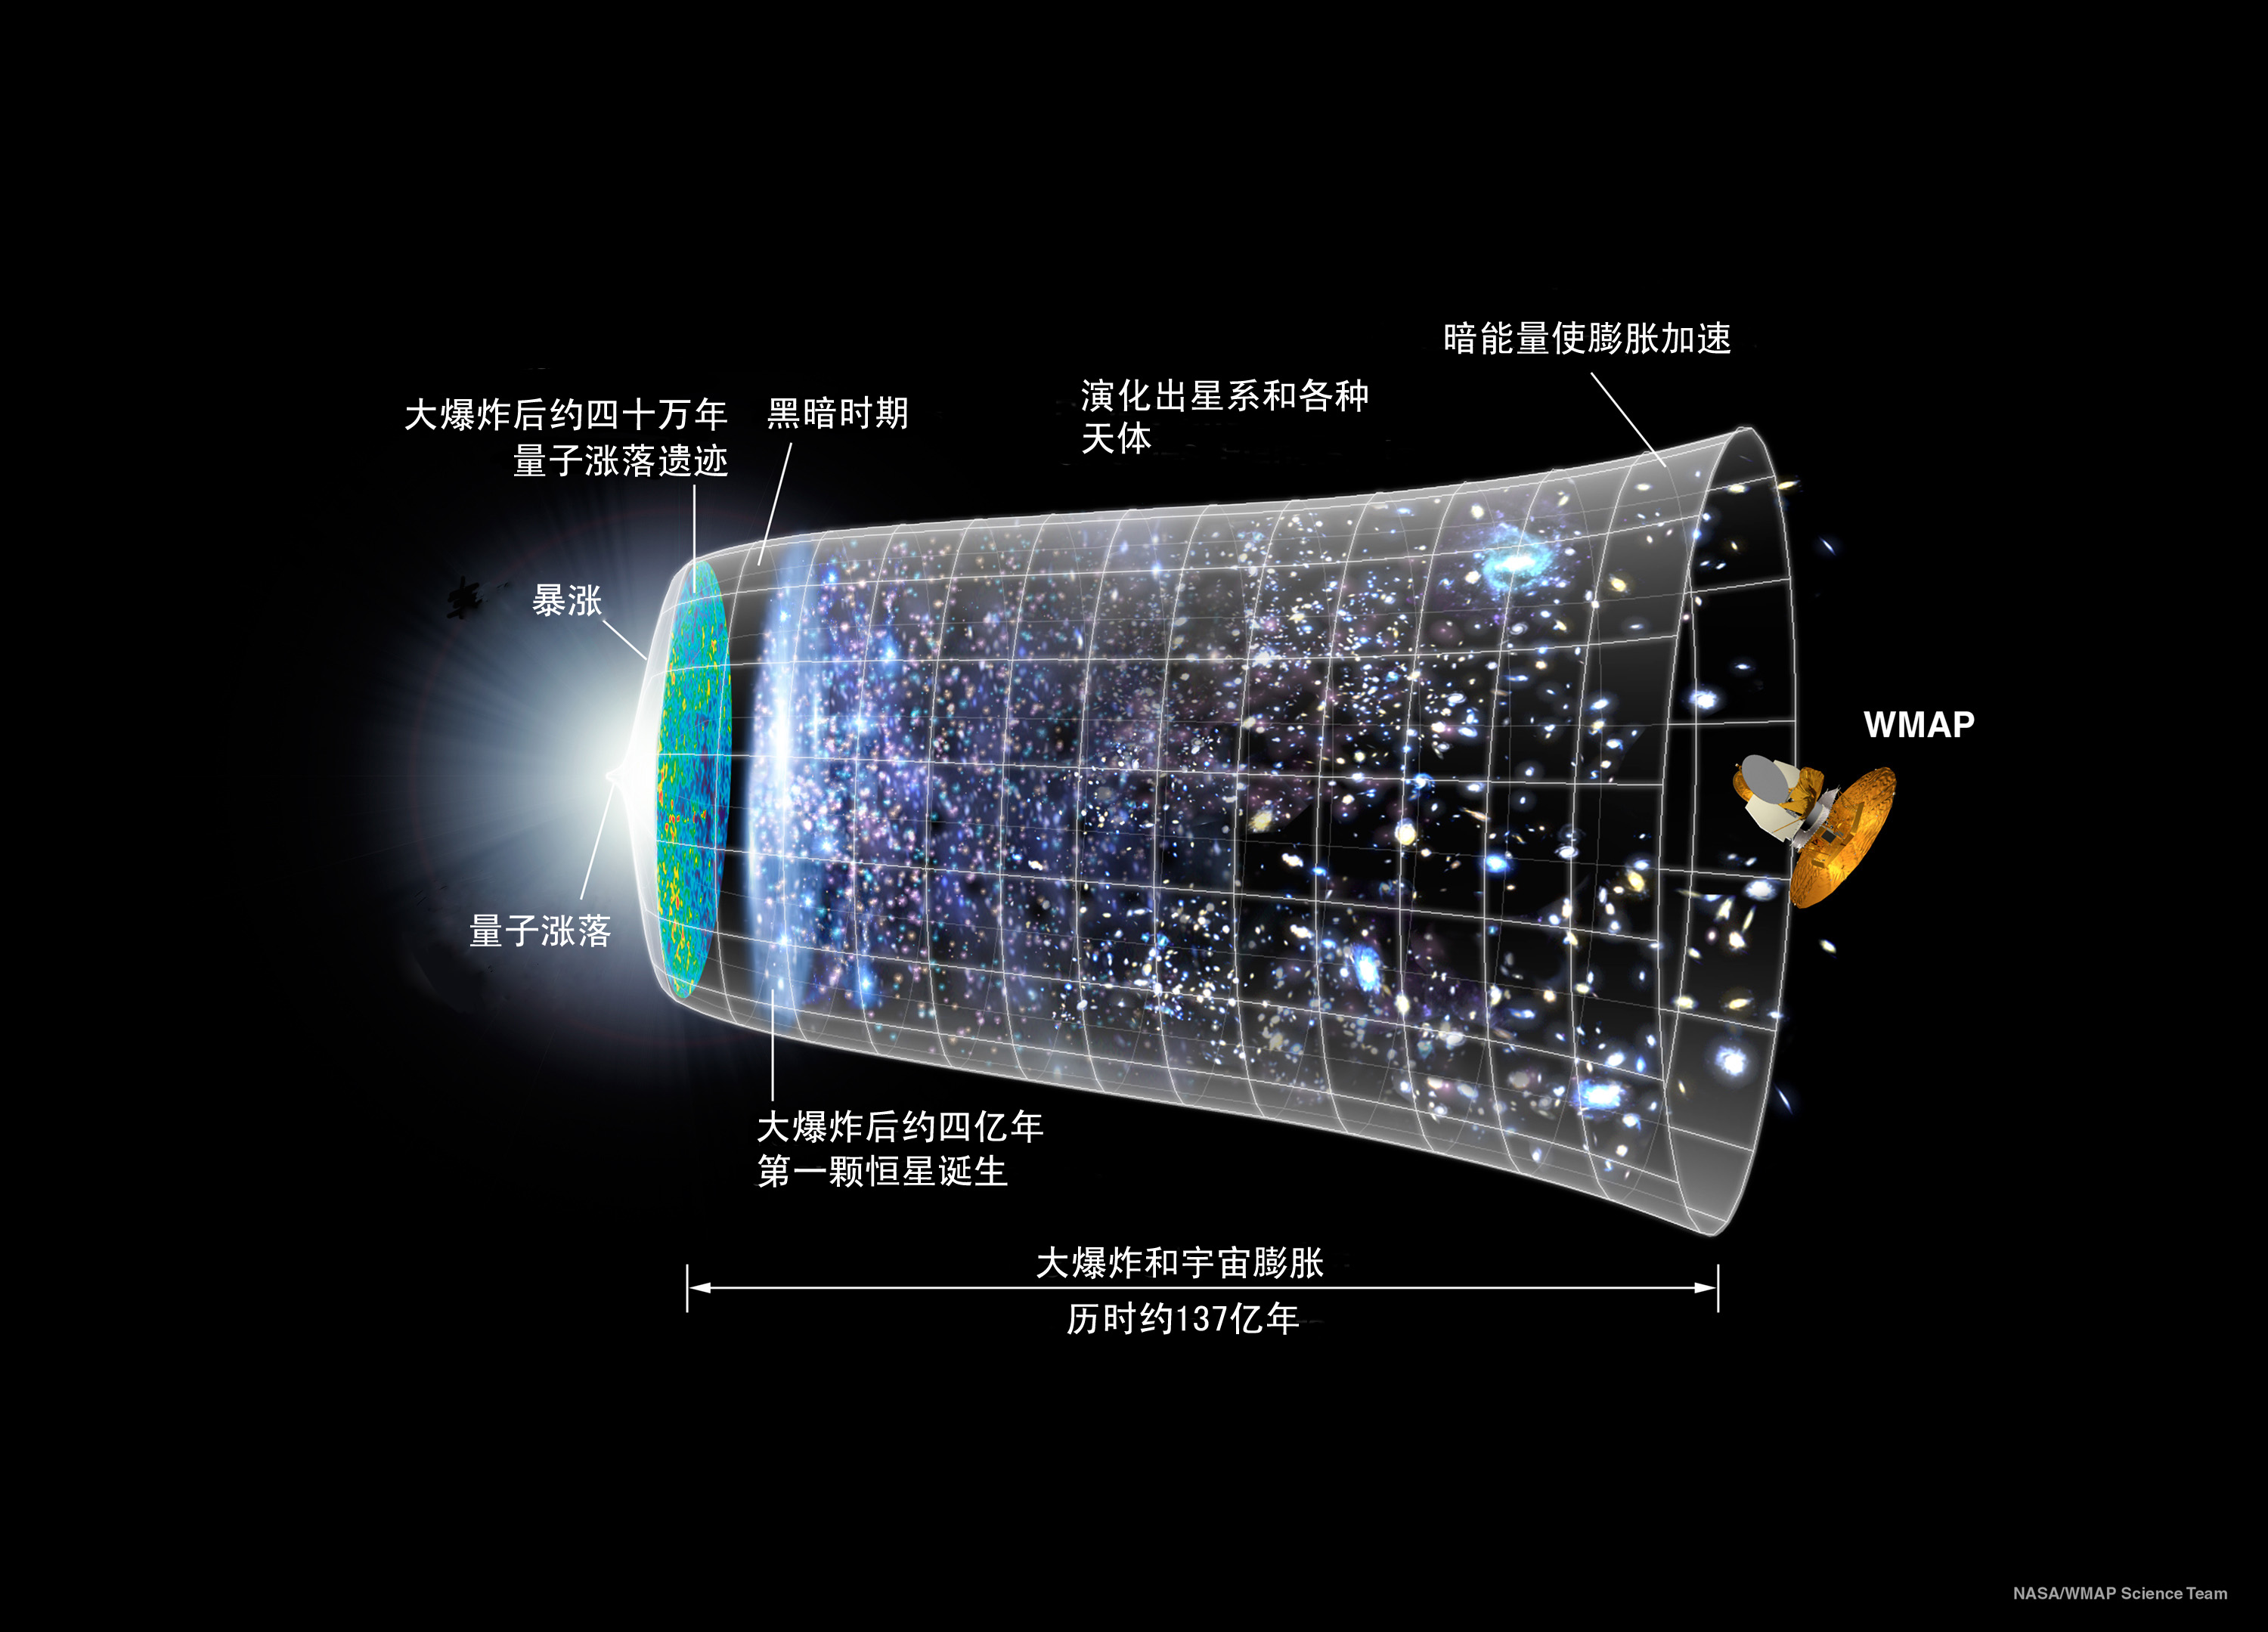
\includegraphics[width=6in]{Img/CMB_Timeline75_zh-cnversion.jpg}
  \caption{宇宙演化的构想图,图片来自2006年WMAP新闻发布会。}\label{fig:history-of-universe}
\end{figure*}

尽管从暴胀的诞生到现在已经有无数个暴胀模型被提出,但是目前为止暴胀的理论起源依旧没有一个统一的结论。
为了尝试给暴胀模型找出背后的理论依据,有人试图把超引力作为一种选择,以其为理论框架,在其中嵌入暴胀模型。超引力暴胀理论到如今已发展了三十多年,各种不同类型的
暴胀模型都已成功在超引力框架内被实现,包括拐点暴胀模型。

暴胀理论还提供了一种产生原初扰动的机制,产生的标量扰动和张量扰动以一种自然的方式解释了CMB中观测到的各项异性以及提供了宇宙大尺度结构能够形成的种子。其中标量扰动的存在已经被CMB各项异性的观测所证实\citep{akrami2018planck}。
大尺度上的张量扰动虽然还未被观测到,但是Planck
2018联合BICEP2/Keck阵列的数据对张标比$r$的上限给出了更紧的限制,在$95\%$的置信水平上$r<0.064$。

一阶扰动理论中,张量扰动满足的运动方程是自由的波动方程。意味着扰动的演化受到宇宙背景演化的直接影响。而在二阶扰动的情况下,自由波动方程获得了一个来自一阶标量扰动的源项\citep{matarrese1998relativistic,acquaviva2002second}。标量扰动在辐射为主时期进入哈勃视界后能够诱导产生二阶引力波。
如果假设标量扰动的功率谱函数是幂指數形式,那么与暴胀期间产生的一阶引力波相比,二阶引力波完全可以被忽略\citep{ananda2007cosmological,baumann2007gravitational},因为根据Planck
2018年的数据,标量谱指标$n_{s}$在$68\%$的置信水平上被限制在$n_{s}=0.9649\pm 0.0042$。
但假若标量功率谱在小尺度上有一个加强的话,二阶引力波的大小甚至可以增大到可以与一阶引力波相比拟,届时便必须考虑它的影响\citep{assadullahi2009gravitational,alabidi2013observable,alabidi2012observable,chen2019pulsar,cai2019gravitational,inomata2019gravitational,cai2019universal}。并且小尺度上功率谱的增强会使得扰动在辐射为主时期进入视界后通过引力塌缩的方式生成原初黑洞\citep{garcia1996density,clesse2015massive,yokoyama1995formation,dalianis2019primordial,gao2018primordial,di2018primordial,garcia2017primordial,garcia2016gravitational}。
因此一阶标量扰动诱导产生的引力波可以用来约束原初黑洞的丰度,反过来原初黑洞的丰度也能用于约束二阶引力波的大小。

此前已经有工作\citep{garcia1702phys}通过单拐点的单场暴胀模型成功使标量谱在小尺度上得到增强。其中用到的拐点暴胀模型是在超引力框架内利用对数K\"ahler势和三次方超势构造得来\citep{gao2015inflection}。近期,又有文章在超引力中基于单手征超场构造出了双拐点暴胀模型\citep{gao2018primordial},其中一个拐点在大尺度上给出满足CMB约束的功率谱,另一个拐点使得功率谱在小尺度上产生一个峰。这个峰的存在使得扰动在辐射为主时期进入视界后能够产生原初黑洞。

基于这个背景,产生了我的第二个工作。在\citep{gao2018primordial}中双拐点暴胀模型的基础上
用解析方法计算二阶诱导引力波的大小,并与LISA和太极的观测灵敏度进行比较,看是否有可能通过诱导引力波的信号是否有可能被探测到。

本文首先将简要介绍现代宇宙学理论,包括标准标准宇宙学、暴胀理论和扰动理论。接下来两章分别介绍整个研究生期间的两个主要工作。文章的具体结构如下。

文章的第二章介绍现代宇宙学标准模型,包括四个部分。第一部分介绍标准宇宙学模型,从宇宙热大爆炸理论到$\Lambda$CDM模型。第二部分介绍暴胀宇宙学,包括历史背景、一般模型以及一些基本概念。
第三部分介绍规范扰动理论,包括扰动的分解、演化以及规范之间的变换。第四部分介绍
扰动功率谱,包括标量扰动以及张量扰动的功率谱的推导。

文章的第三章介绍超引力框架下的单拐点暴胀模型,包括三个部分。第一部分简单介绍了基于超引力的暴胀理论的历史,包括超引力暴胀模型发展过程中遇到的一些问题以及解决方法。第二部分介绍了跑动动能暴胀模型,包含跑动动能暴胀模型提出的背景,以及这一类暴胀模型的基本特点。第三部分介绍了本人的第一个工作,在超引力框架下,
通过选取特定形式的超势$W$,并对参数进行微调得到了具有单个拐点的标量势能。并以
Planck 2015
数据中曲率扰动的大小作为约束条件,计算了多种参数取值下的$n_{s}-r$的预测值,
并将其与 Planck 2015 数据进行了比较,发现与观测较为符合。

文章的第四章介绍了双拐点暴胀模型与引力波,包括四个部分。第一部分介绍了一般的双拐点暴胀模型,及其特点。第二部分首先介绍了超引力下的单场暴胀模型,
然后通过选取满足约束条件的超势构造了一个单场暴胀模型,并且在暴胀结束会得到一个恢复超对称的闵可夫斯基真空。进一步在参数空间中调节超势中引入的几个参数值,将构造出
具有双拐点的暴胀模型。第三部分给出了所构造的双拐点暴胀模型对应的功率谱,由于拐点的
存在,包含慢滚参数的计算功率谱的近似公式将不再适用,因而采用数值方法求解MS方程。
% 第四部分简单介绍原初黑洞,根据原初洞的生成机制以及观测数据,调节功率谱中峰的位置以及幅度。
第四部分根据数值计算得到的标量功率谱计算诱导引力波的能量谱,并将其与LISA\citep{amaro2017laser}和太极\citep{guo2018taiji}的期望灵敏度曲线进行比较。对功率谱进行函数拟合后,对得到的结果进行了一定的推广讨论。
最后一章总结。
